\chapter{Tablet Method}
\label{TabletMethodChapter}

\section{Abstract}

A methodology is proposed that allows for experiments of colour constancy to be performed in real and complex environments, in order to better understand colour constancy in the real world. The methodology considered uses a tablet computer to present a spatial version of an achromatic point selection task. 
The key concerns are whether such a methodology can record differences in perceptual white point, present a stable stimulus across disparate environments, and be suitable for naive observers following minimal instruction. On each point, the method is shown to be at moderately successful, with caveats, and suggestions are provided for improvements.
If judged satisfactory, such a methodology could be used to investigate the effect of multiple cues, conflicting cues and cues which cannot easily be reproduced in a controlled in a lab environment.

\section{Introduction}

To further our understanding of colour constancy, investigators have traditionally designed experiments where the number of variables compared to a real-world environment is greatly reduced. This allows investigators to carefully query the impact of any individual variable, or the interplay of a small number of variables. An example may be the `Mondrian' patterns used in a vast number of investigations, most famously used by \citet{land_retinex_1964} (and well described by \citet{hurlbert_colour_1999}) where an observer is presented with a flat and unmoving selection of overlapping coloured rectangles in place of a real scene, or the more recent experiments of \citet{kraft_mechanisms_1999} where objects representing potential colour constancy cues (such as a tin-foil covered cone) were removed from a neutrally coloured box one-by-one in order to probe their relative usefulness.

\begin{figure}[hbp]
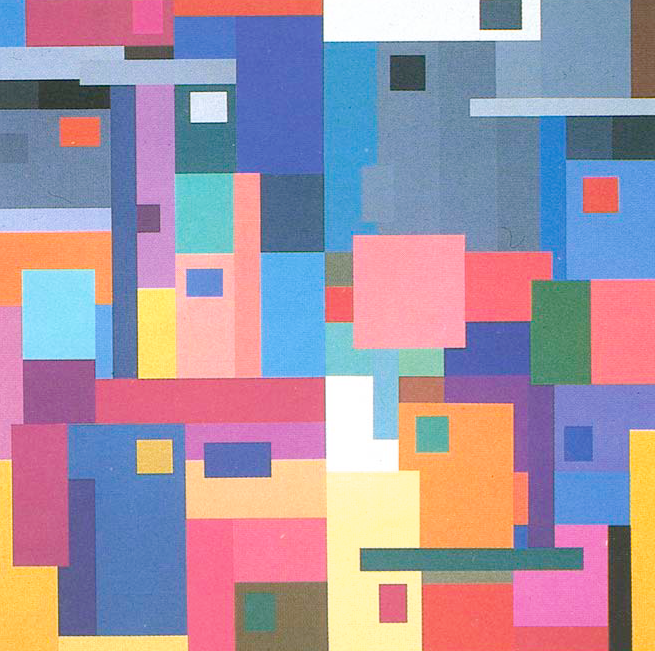
\includegraphics[width=\textwidth]{figs/tablet/mondrian.png}
\caption{An example `Mondrian', reproduced from \citet{land_recent_1986}.}
\label{fig:mondrian}
\end{figure}

\begin{figure}[hbp]
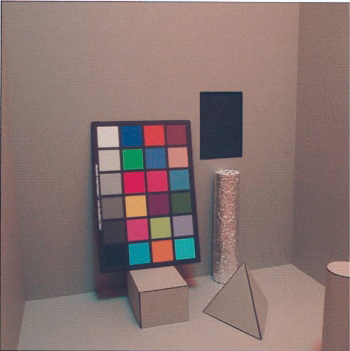
\includegraphics[width=\textwidth]{figs/tablet/KraftBrainard.png}
\caption{A colour constancy experiment investigating the roles of multiple cues, reproduced from \citet{kraft_mechanisms_1999}}
\label{fig:KraftBrainard}
\end{figure}

Simple experimental stimuli allow for clear questions to be asked, and for those questions to be answered with statistical strength. Such research is valuable. However, the use of simplified stimuli risks overlooking unknown scene attributes, and the human behaviours which may be reliant on them. Recent experiments (ref) have found that colour constancy in lab environments is never ‘complete’; is this representative of real world behaviour or could this result be due a lab environment failing to deliver all the cues available to an observer in a natural environment? Recent technological advances have enabled experimenters to reproduce natural scenes with increasingly accuracy and comprehensiveness \citep{heasly_rendertoolbox3_2014}, but the number of variables in real scenes is practically infinite, and whilst our ability to reproduce a scene increases, we only reproduce what we deem important at the time. Using a real-world environment would allow for processes to occur as they would do naturally, in the environment for which these processes are presumably optimised (See \citet{kelly_chips_2017} (poster ref, try to replace) and \citet{shepard_perceptual_1992}.)

There are two clear challenges to the use of natural environments for scientific study; the inability to control target variables, and the influence of uncontrollable or uncontrolled non-target variables. The first may be surmountable; depending on the variable in question it might either be controlled by force, or over time natural variability may provide the required experimental range. The second may be insurmountable but, depending on the specific situation, it may be permissible to consider uncontrolled variations simply as sources of experimental noise. Further challenges arise where connections exist between target and non-target variables, or where the influence of the non-target variables dwarf the effect of the target variable.

One further challenge: it is rare for an experiment in a real-world environment to not intrude onto that real-world scene and change it in some way. The only true solution to this problem would be to consider unannounced observation of a natural behaviour as the only acceptable scientific method. A pragmatic compromise is to design an experiment such that it modifies the environment of the observer minimally, and to carefully consider the impact that the experimental set-up may have upon observers.

The method presented here is a variant of the `achromatic setting' method. For overviews see `achromatic adjustment' in \citet{foster_color_2011} and `Matching to an internal standard' or `achromatic setting' in \citet{smithson_sensory_2005}. The proposed variation should allow for use in real-world environments, whilst minimally influencing the observers’ state of chromatic adaptation. The achromatic setting method requires an observer, under specific conditions, to adjust the chromaticity of an item in their visual field such that this item appears achromatic. Changes in selected achromatic point (in colour space) are thought to represent general adaptive shifts. For example, an observer in a uniform and strongly chromatic environment would be expected to pick an achromatic point which is shifted towards the chromaticity of that environment, compared to the achromatic point which they might select in a more neutral environment. 

This is often practically achieved by having the object be an area of a computer screen, and have it controllable in two or more dimensions (such as unique red/green and blue/yellow). 
In the spatial achromatic point setting method, as presented here, a tablet computer is given to an observer to hold as is comfortable to them, and upon this computer appears an isoluminant slice through a nominally perceptually uniform colour space, from which they are requested to select (by touching upon the screen with a finger) the point which they deem to be most achromatic (the specific phrase `grey-est or least colourful' is employed in order to make the task suitable for non-colour-scientist observers). The term ‘spatial’ is used since the user provides information through making a spatial selection which directly corresponds to a colour choice, where in other methods abstract sliders or knobs may be used as input mechanisms.

To minimise the effect of the presentation of chromatic scenes upon the viewer, which may influence an observer’s state of chromatic adaptation, this process is repeated a number of times with the area of colour space which is presented varying, through random rotation about the luminance axis, and ransom offsetting through both dimensions of the chromatic plane.
In this chapter I will outline the procedure, and describe some experiments performed to explore the potential and limitations of such a method.

\section{Materials and Methods}
\subsection{Stimuli}

Participants undertook the experiment upon a Dell Latitude 10 ST2 tablet computer with ‘BROTECT’ Matte Screen Protector (223x126mm active screen area, 1366x768 pixels) as described elsewhere \citep{garside_estimating_2016}. This tablet was chosen for its ability to run a Windows environment, and the matte screen protector was added to reduce the severity of specular reflections. 

\begin{figure}[hbp]
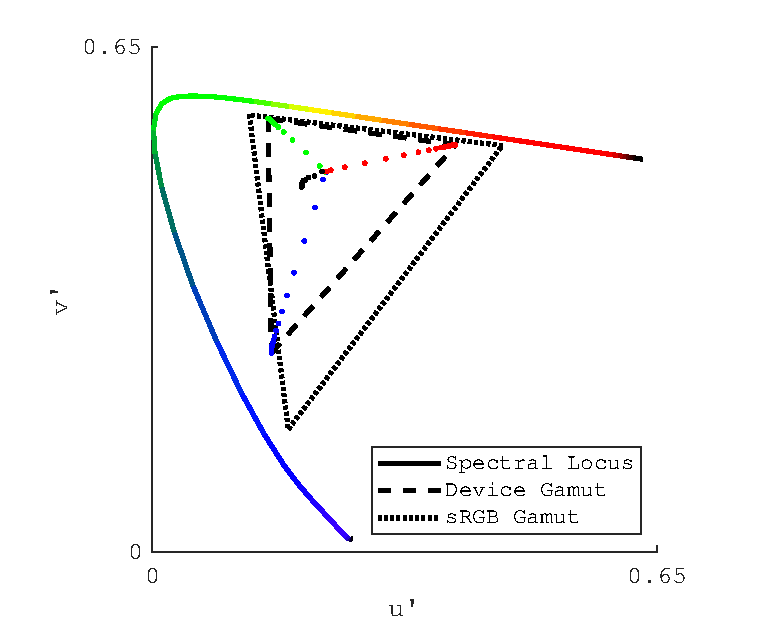
\includegraphics[width=\textwidth]{figs/tablet/gamut.pdf}
\caption{The display gamut. Red, green and blue dots indicate chromaticities of single channels at different pixel values. The black dots are the chromaticities achieved when the pixel values are kept in line for each channel. This can be described as the native white point of the display.}
\label{fig:gamut}
\end{figure}
% Generated using the 'Plot gamut' section of SAPS_TabletCharacterisation.m

The stimulus presented to observers was an isoluminant plane (in CIE L*) through CIELUV colour space. CIELUV was chosen for having an associated object colour space, where comparisons between the chromaticity of light sources and the chromaticity of selections could be made. The stimulus was specified as: L*: 60 uniformly across field, u*: ranging linearly from -50 to 50 from one side of the field to the other, and v*: as for u*, but along the perpendicular axis, so that the stimulus was of uniform lightness and smoothly changing hue and chroma. The stimulus created was 2188 pixels square; this is larger than the pixel dimensions of the screen to allow for the stimulus to be rotated freely and offset by up to a third of the image in any direction before the edge of the image is encountered. [include maths?]

The stimulus was specified with the above attributes in a matrix within MATLAB. CIELUV values were converted to XYZ tristimulus values using built in functions, with reference white set as the XYZ tristimulus values of the display at maximum white (with screen protector), as measured with an Xrite…. Linearisation was achieved through the use of a look-up table, computed by spline interpolation of the measured outputs at 15 pixel (KT: pixel drive value?) value increments from 0 to 255 for each channel. The stimulus was then output as an 8-bit tiff image, which could be easily loaded and manipulated by the psychophysical stimulus presentation software PsychoPy \citep{peirce_psychopypsychophysics_2007}. (Illustrate with flow diagram?)

\begin{figure}[hbp]

\includegraphics[width=\textwidth]{figs/tablet/stimulus.png}
\caption{Full stimulus image.}
\label{fig:Stimulus}
\end{figure}
% Copied and pasted from original psychopy folder. Could regenerate using stimulusGenerator002.m

A program in PsychoPy was written (code ref) that presents the stimulus 30 times, with random rotation and random offset in the horizontal and vertical dimensions of between -1/6 and +1/6 of the respective dimension. Thus ‘objective grey’, where [u*,v*] = (0,0), was always within the central third (in each dimension) of the screen. This program saved details of the offset and rotation (‘dpX’, ‘dpY’ and ‘ori’), coördinates of observer selected point (‘x-co_raw’, ‘y-co_raw’, and also ‘direction_raw’, ‘magnitude_raw’), and time taken to make selection, measured since last selection (‘toc_raw’).

The effect of rotation and offset was that on each stimulus presentation the observer saw a stimulus that appeared somewhat different to the previous stimulus, but still hopefully included their preferred achromatic point. The rotation and offset can be illustrated by plotting the chromaticities present in any one stimulus presentation, as in figure X. Plotting the chromaticities present across a full run of 30 trials yields figure Y, where it can be seen that the rotation results in a roughly circular spread of chromaticities, and the rotation and the offsetting together result in a gradient of likelihood of presentation which is high at the centre of the full stimulus and lowest at the edges of the full stimulus. This gamut distribution is referred to further in the text as the `practical gamut'.

% Single shot figure needed

% \begin{figure}[hbp]
% \includegraphics[width=\textwidth]{figs/tablet/????}
% \caption{A representation of the chromaticities present in a single stimulus. Note that the gamut is not rectangular for 2 reasons: firstly, because CIELUV is not a linear transformation of CIE u’v’ , and secondly because for this particular stimulus, the bottom left corner (as presented above) intersects with the display gamut boundary, resulting in a gamut compression to that corner.}
% \label{fig:?????}
% \end{figure}

\begin{figure}[hbp]
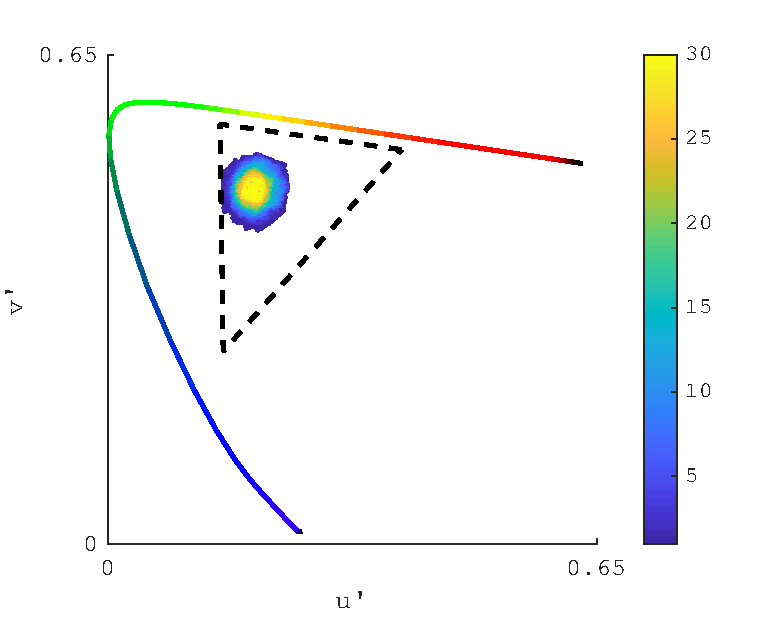
\includegraphics[width=\textwidth]{figs/tablet/practical_gamut.pdf}
\caption{: The `practical gamut'. This plot shows the relative frequency that chromaticities are presented. The highest number of times a particular chromaticity can be presented is 30, since there are 30 trials. As described in the main text, chromaticities falling towards the specified objective white point of the stimulus are presented every stimulus, whereas those further away from the centre of the stimulus are presented less frequently.}
\label{fig:practical}
\end{figure}

\begin{figure}[hbp]
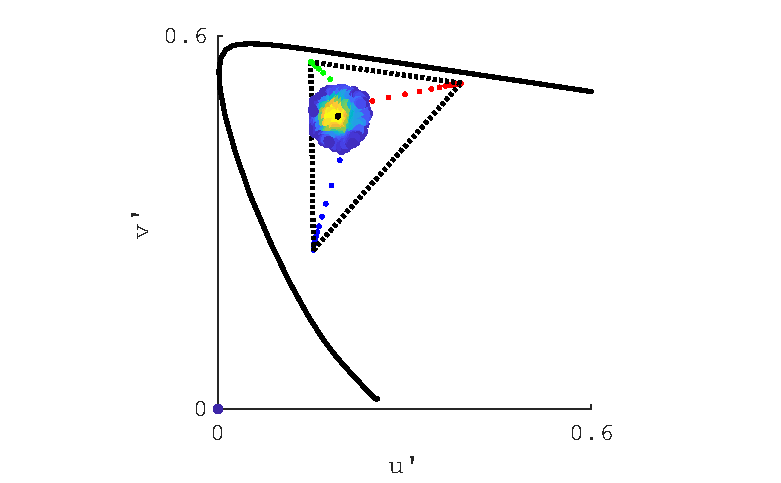
\includegraphics[width=\textwidth]{figs/tablet/practical_gamut2.pdf}
\caption{The `practical gamut' within the context of the display gamut.}
\label{fig:practical2}
\end{figure}

\section{Observer Task and Ethics}

For one of the experiments reported here, observers were selected randomly from visitors to The British Museum. As a precursor to this, a short pilot session was conducted in The Grant Museum of Zoology. See section 3.4 for further details on locations.
For both museum studies, a visitor would be approached by the experimenter (DG) and asked whether ‘they would be interested in taking part in a colour vision experiment’. Those who replied positively were verbally informed of the ethics details for the study, the principal parts of which were: that no identifying information would be recorded, that the experiment carried no risks greater than those associated with normal use of a tablet computer, that observers were not paid or otherwise incentivised to take part, and that the task would take roughly ten minutes. This study was approved by the UCL Ethics committee: Project ID Number: 9357/001. [Appendix X]

For other trials reported here where the location was ‘UCL PAMELA’, participants were recruited from the author’s friends and family, with the hope that this would assure attendance and motivation and to take advantage of short-notice availability of the experimental space. Participants were informed of the ethics details for the study in advance of attending. Ethics approval was provided following the amendment of the aforementioned ethics application (9357/001).

In all cases, the observer was instructed to hold the tablet such as was comfortable for them to do so, upon which the first trial of the experiment was already visible. They were instructed to ‘touch the grey-est, or least colourful, point on the screen’. Most observers seemed to find this task initially difficult, but within the first few trials seemed to develop an increased comfort and ease with the task, which resulted in a decreased response time (Illustrate with graph of response time?). At this point the observer was told that there would be thirty trials. No training was provided, and no runs were excluded as training runs.

\begin{figure}[hbp]
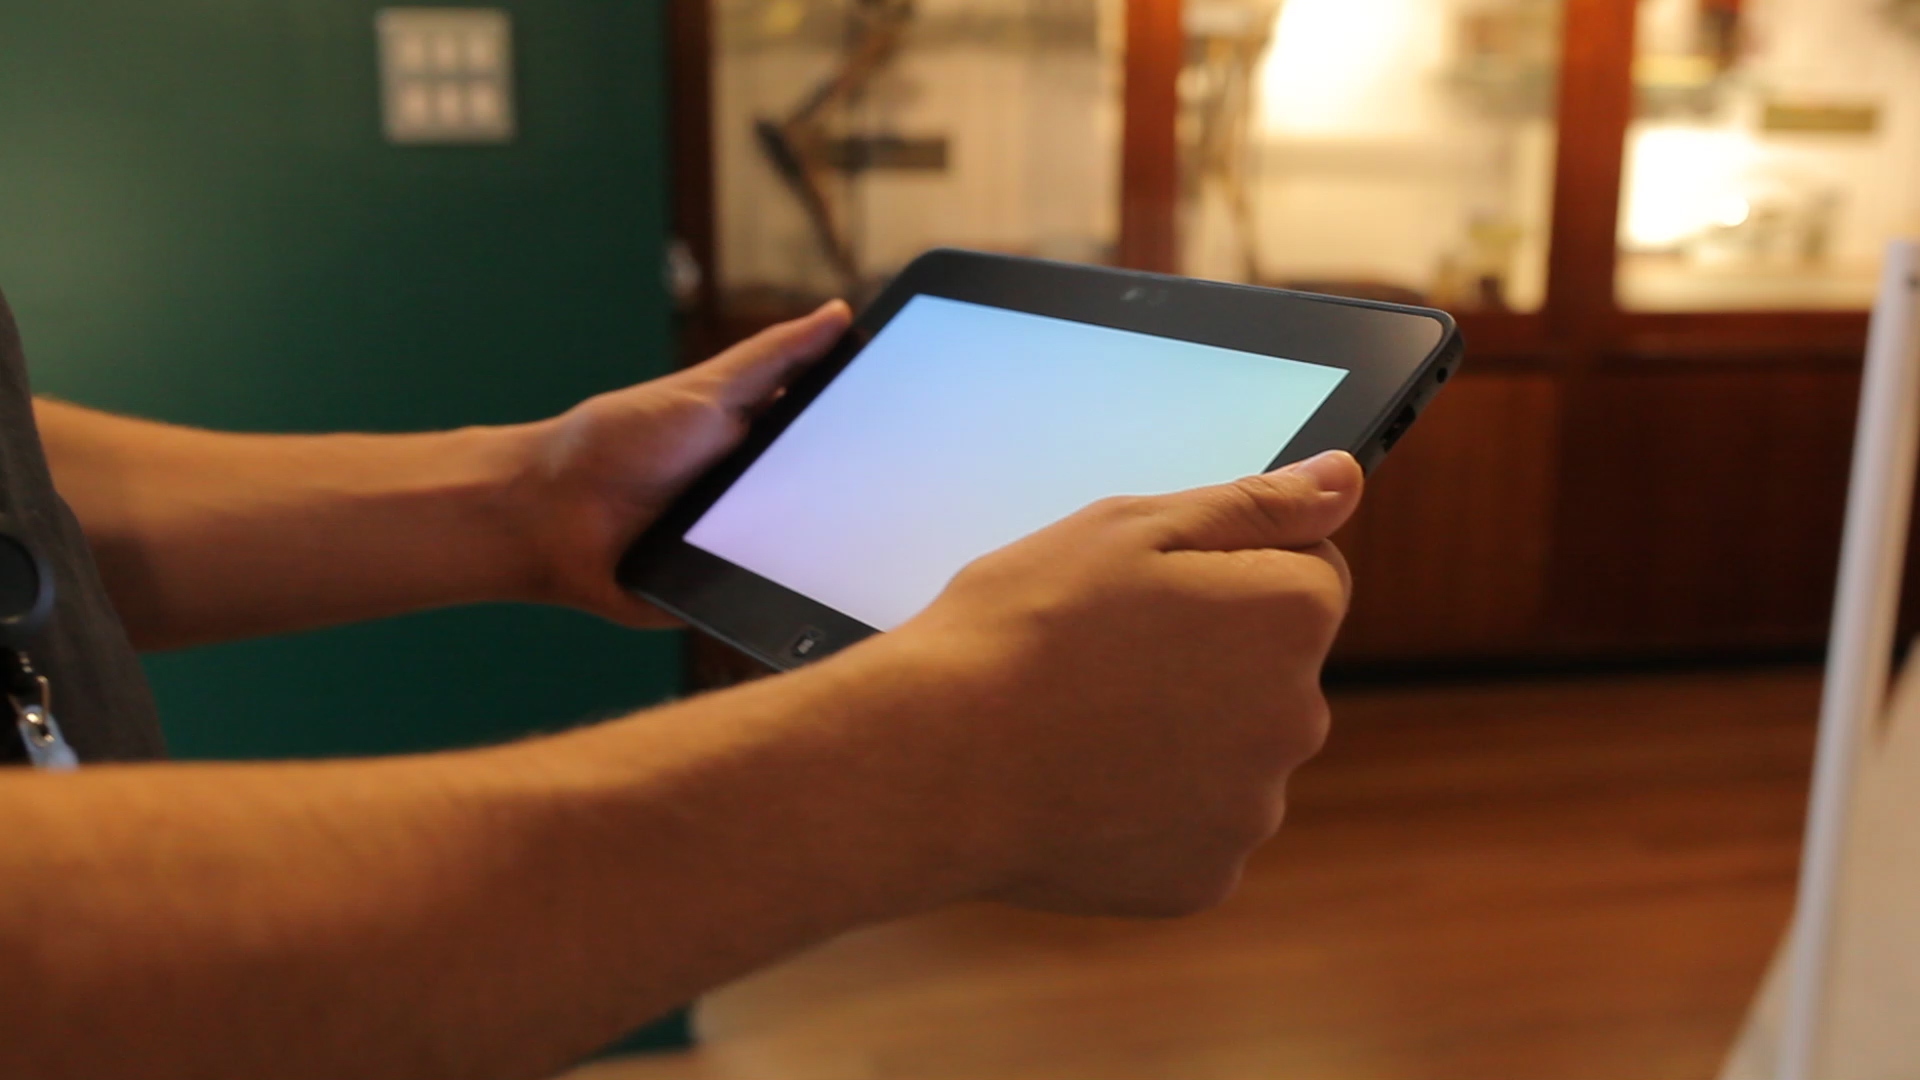
\includegraphics[width=\textwidth]{figs/tablet/MVI_3213-1.jpg} % E:\Pictures\2016\2016-10-14
\caption{Photo of participant (author) holding tablet.}
\label{fig:grant_demo}
\end{figure}

\begin{figure}[hbp]
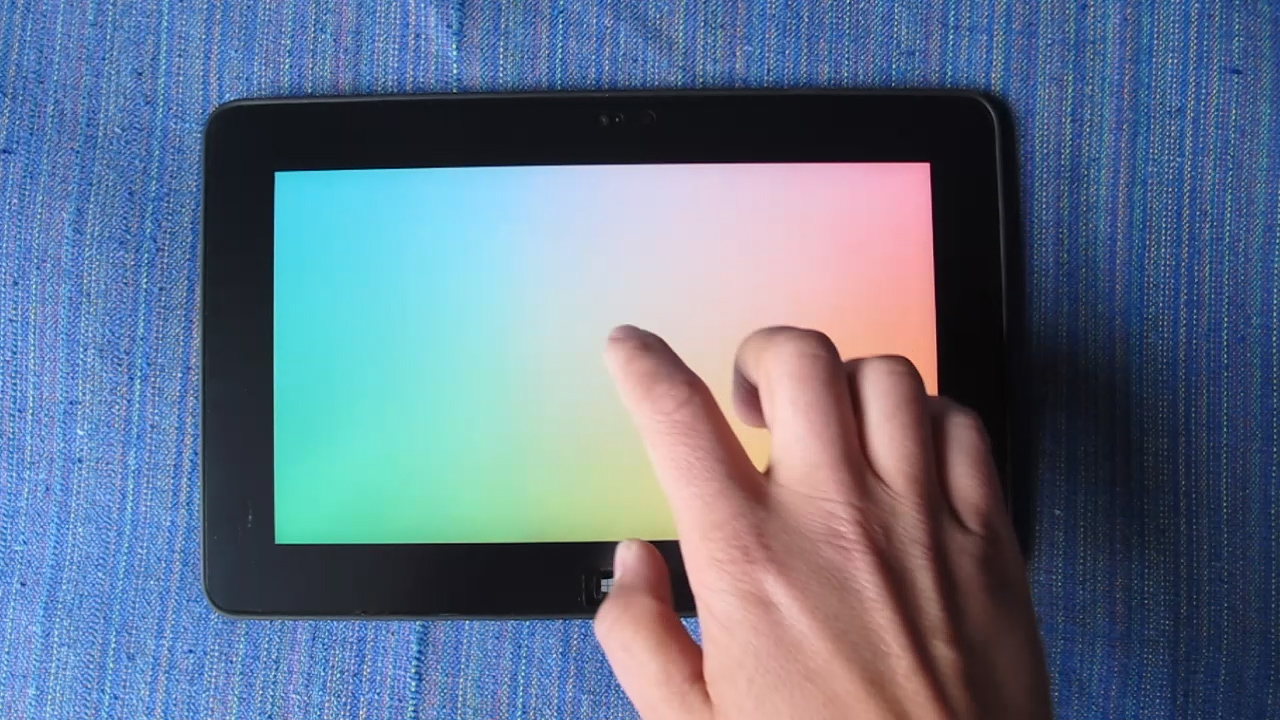
\includegraphics[width=\textwidth]{figs/tablet/MVI_3889-4.jpg} % E:\Pictures\2016\2016-10-18
\caption{Photo of stimulus on tablet and finger in motion towards subjective point of achromacy.}
\label{fig:finger}
\end{figure}

Following the thirty trials, a secondary task was presented to observers, designed to characterise their touch input. This task features a 2x2 checker board (+image) pattern upon a black background. Observers were instructed to touch the centre of this checker board. Upon registering a touch, a new checkerboard would be presented, of the same attributes but modulated in position in the same way as the main stimulus (rotated randomly and offset by up to 1/6 of the screen dimensions in either vertical or horizontal directions). This data was later used to calibrate touch input, and to ascertain the amount of measurement uncertainty derived from touch input. 

\begin{figure}[hbp]
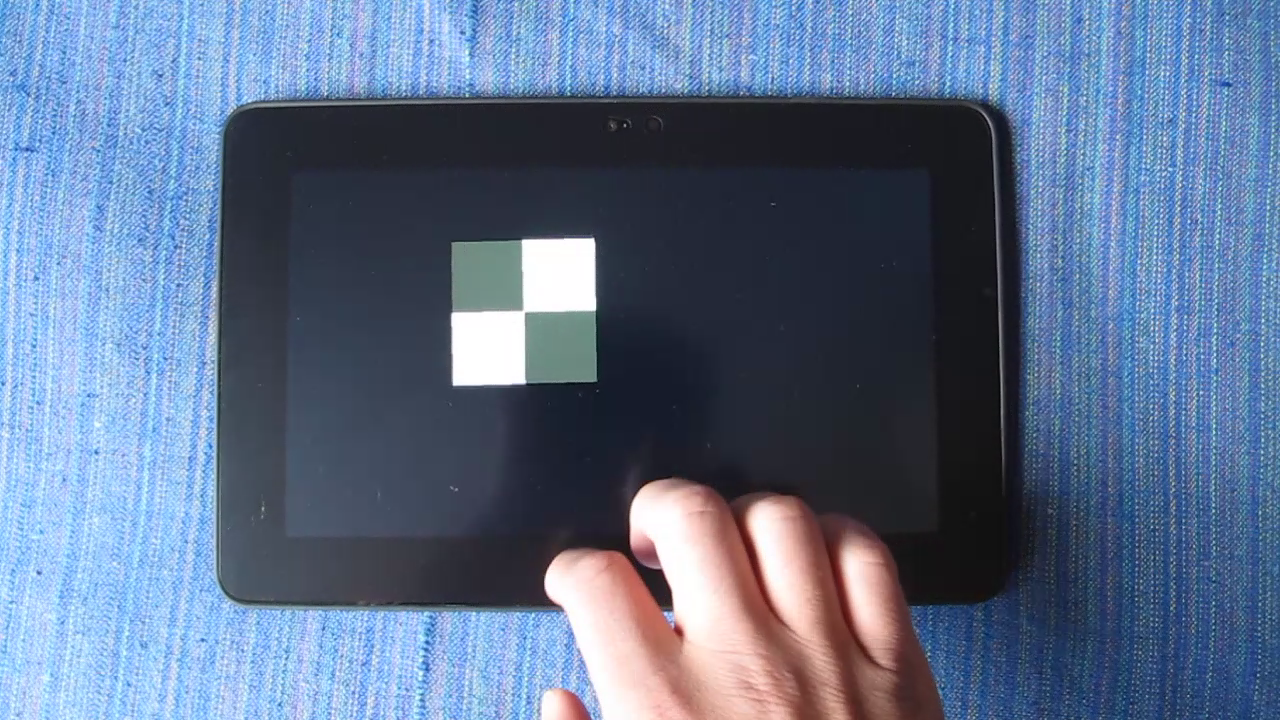
\includegraphics[width=\textwidth]{figs/tablet/checker_board.png} 
\caption{Photo of checkerboard task. Participant is requested to touch centre of the checkerboard pattern.}
\label{fig:checkerboard}
\end{figure}

%Doing this without incentive for participants meant that it was rushed (?)

\section{Data Analysis}

The data was analysed in MATLAB using the following pipeline:
\begin{itemize}
\item Data loaded into MATLAB from an excel file
\item Spatial touch points calibrated using touch characterization data
\item Spatial data converted into chromaticity data
\item Data graded for performance and exclusions introduced where appropriate (see section 5.2.1 for further details) %!!!!!!!!!!!!!!!!!!
\item Data plotted either as:
\begin{itemize}
\item Full dataset scatter
\item Standard deviation ellipse/line plotting (based on code from ) %!!!!!!!!!!!!
\item Dataset mean plotting (only where number of participants was large)
\end{itemize}
\end{itemize}

Data was considered in comparison to a baseline dataset, consisting of the results of a theoretical trial where an observer touched the spatial centre of the screen each time (further details in section 5.1), and a practical gamut which describes the frequency with which each chromaticity was presented to the observer (See section 3.1 for further discussion of this).
%Demo plots?

\section{Environments}
\subsection{UCL Grant Museum of Zoology}

The UCL Grant Museum of Zoology is a natural history museum within University College London (UCL) with ‘over 68,000 specimens’ [14], which is open to the public and also used as a teaching resource. It is lit with a mixture of daylight and LED lighting, and a rarely used fluorescent lighting system (not used during any experiments).
This space was used for preliminary experiments. 

\begin{figure}[hbp]
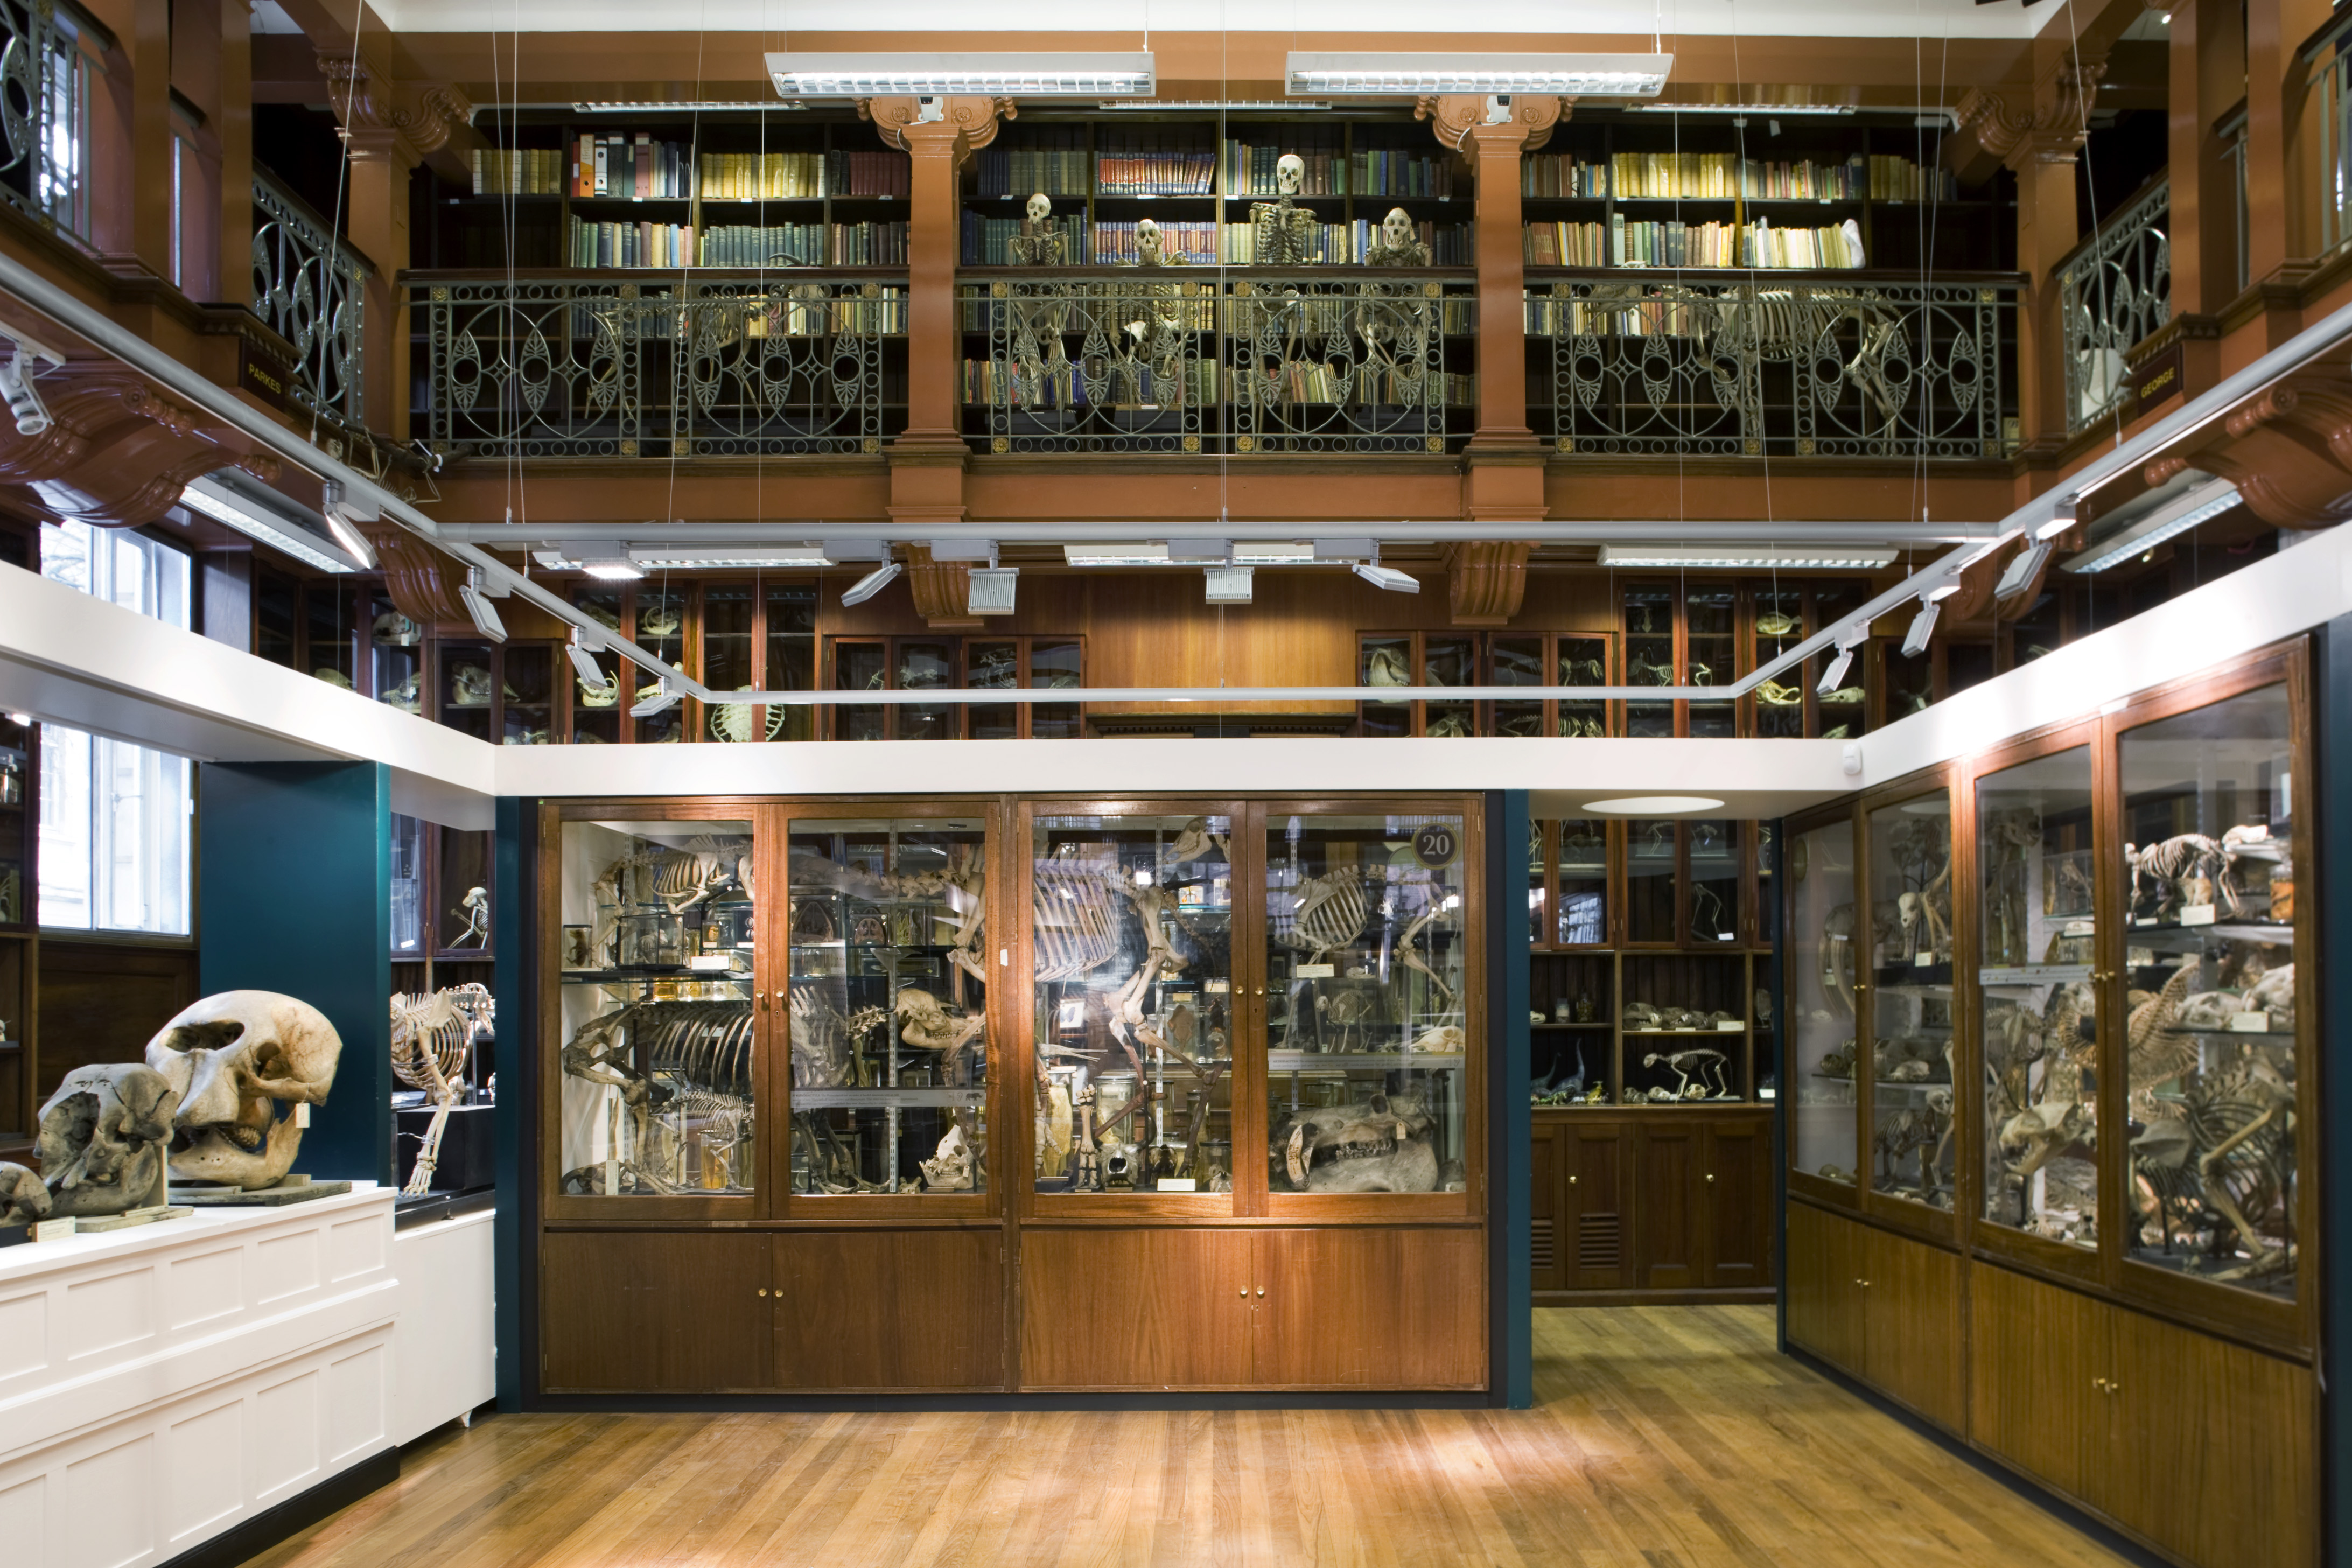
\includegraphics[width=\textwidth]{figs/tablet/grant.jpg} 
\caption{The central space at the UCL Grant Museum of Zoology. Note the daylight on the left, the LED lighting at mid-height and the fluorescent lighting at the very top of the image. Image copyright: UCL and Matt Clayton.}
\label{fig:grant}
\end{figure}

\subsection{The British Museum}

The British Museum is a large museum located close to the main UCL campus, which exhibits artefacts of artistic, cultural and historical relevance. 

Three spaces within the museum were used (with permission):

\begin{enumerate}
    \item Rooms 77/78 (‘Greek and Roman Architecture’, ‘Classical Inscriptions’), lit with fluorescent lighting.
    \item Room 25 (‘Africa’ – specifically the east section of the room), lit with tungsten  lighting.
    \item The Queen Elizabeth II Great Court, lit with filtered daylight \cite{foster_and_partners_london._great_2002} during daylight hours, with additional lighting at twilight and after sunset. All experiments were carried out during daylight hours, where additional artificial lighting was not employed.
\end{enumerate}

% Photos of spaces























